\documentclass[aspectratio=169]{beamer}
\setbeamertemplate{navigation symbols}{}
\usepackage{color,amsmath,comment, subfigure}
\usepackage{booktabs}
\usepackage{url}

%%%%%%%%%%%%%%%%%%%%%%%%%%
\title[]{The connected age and the small world problem}
\author[]{Social Networks (Soc 204)\\Spring 2021\\Princeton University}
\institute[]{Matthew J. Salganik}
\date[]{Week 1, Lecture 2\\ Video 1/3: Introduction

\vfill

\begin{flushleft}
\vspace{0.7in}

\includegraphics[width=0.05\textwidth]{figures/cc.png}
\end{flushleft}
}

\begin{document}
%%%%%%%%%%%%%%%%%%%%%%%%%%%
\frame{\titlepage}
%%%%%%%%%%%%%%%%%%%%%%%%%%%
\begin{frame}

Expectations about reading and lecture:
\begin{itemize}
\item I expect you to watch the pre-read video
\pause
\item I expect you to read the materials
\pause
\item In the videos, I will do a mix of reviewing the reading, providing context, and discussing extensions 
\end{itemize}

\end{frame}
%%%%%%%%%%%%%%%%%%%%%%%%%%%
\begin{frame}

\begin{columns}
\begin{column}{0.5\textwidth}
  \begin{center}
    
\includegraphics[width=0.50\textwidth]{figures/watts_six_2003_cover}
  \end{center}
\end{column}
\begin{column}{0.5\textwidth}  
\pause
    \begin{center}
     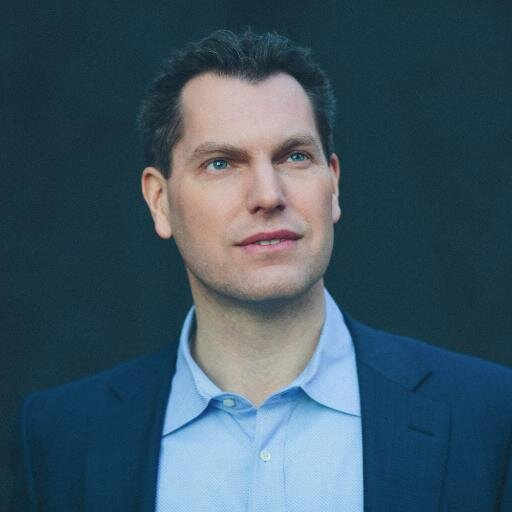
\includegraphics[width=0.5\textwidth]{figures/duncan_headshot}
     \end{center}
\end{column}
\end{columns}

\note{
This book has an author.  He is just a normal person.  I love this book because it shows science in action.  So, when stuff from our precept turns out messy or unexpected that's normal.  This book shows what science is really like: being stuck and confused a lot.
}

\end{frame}
%%%%%%%%%%%%%%%%%%%%%%%%%%%
\begin{frame}

\begin{center}
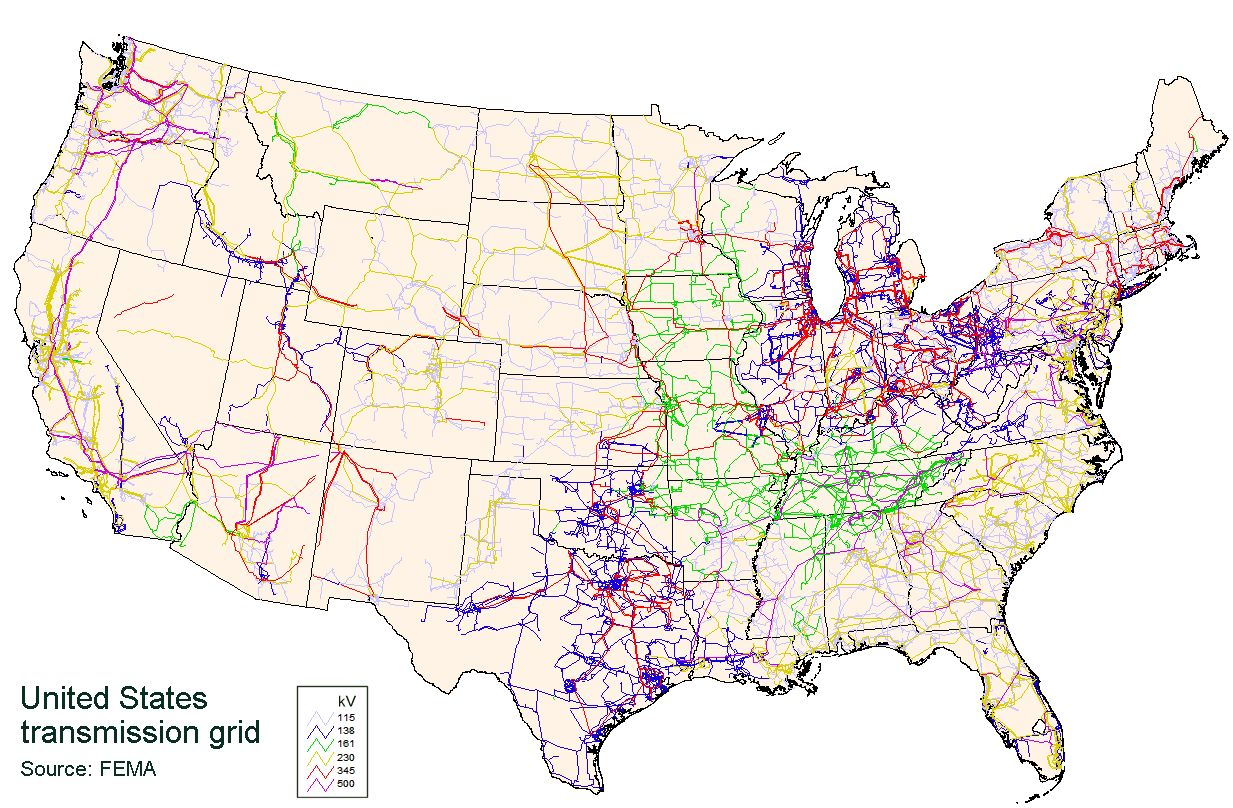
\includegraphics[width=0.8\textwidth]{figures/power_grid}
\end{center}

\vfill
\tiny{\url{https://commons.wikimedia.org/wiki/File:UnitedStatesPowerGrid.jpg}}

\note{
cascading failure in power grid
cascading failure in the financial system.  Government bails out AIG 85 billion dollars.  They do it because 
}

\end{frame}
%%%%%%%%%%%%%%%%%%%%%%%%%%%
\begin{frame}

\begin{center}
\Large{
How does individual behavior aggregate\\ to collective behavior?
}
\end{center}

\note{
Sociology is about: Dog and pack of dogs
Jury members of Juries
Crickets and packs of crickets (how are these crickets connected together)?
}

\end{frame}
%%%%%%%%%%%%%%%%%%%%%%%%%%%%


\end{document}
